\scanpage{150}
\[
\operatorname{pr}_2^!(G_\bullet)\longrightarrow\deleted{\unsure{\unsure{\underline{D}|D}_Z\unsure{\underline{D}|D}_Z}}\operatorname{pr}_2^!(\deleted{G_\bullet}\inserted{\unsure{\underline{D}|D}_Y(\unsure{\underline{D}|D}_Y(G_\bullet))})\xrightarrow{\sim}\unsure{\underline{D}|D}_Z\operatorname{pr}_2^*(\unsure{\underline{D}|D}_Y G)
\]
\inserted{iso si $\unsure{\underline{D}|D}_Y(G_\bullet)$ à ch.\ const.}

d'où
\diagram{\begin{tikzcd}[ampersand replacement=\&,column sep=small]
\mathbb{R}\mathcal{H}om(\operatorname{pr}_1^*(F_\bullet),\operatorname{pr}_2^!(G_\bullet))\arrow[r]\&\mathbb{R}\mathcal{H}om(\operatorname{pr}_1^*(F_\bullet),\unsure{\underline{D}|D}_Z\operatorname{pr}_2^*(\unsure{\underline{D}|D}_Y G))\arrow[d,phantom,"\simeq" description]\\
\&\unsure{\underline{D}|D}_Z(\operatorname{pr}_1^*(F_\bullet)\overset{\mathbb{L}}{\otimes}\operatorname{pr}_2^*(\unsure{\underline{D}|D}_Y G))
\end{tikzcd}}

Il suffit de décrire maintenant
\[
\unsure{\underline{D}|D}_Z(\operatorname{pr}_1^*(F_\bullet)\overset{\mathbb{L}}{\otimes}\operatorname{pr}_2^*(\unsure{\underline{D}|D}_Y G)))\unsure{\text{---}|\longrightarrow}\unsure{\underline{D}|D}_Z\mathbb{R}\mathcal{H}om^\bullet(\operatorname{pr}_2^*G,\operatorname{pr}_1^!(F_\bullet))
\]
\deleted{\unsure{i.e.}} ou encore un hom
\[
\mathbb{R}\mathcal{H}om^\bullet(\operatorname{pr}_2^*(G),\operatorname{pr}_1^!(F_\bullet))\longrightarrow\operatorname{pr}_1^*(F_\bullet)\overset{\mathbb{L}}{\otimes}\operatorname{pr}_2^*(\unsure{\underline{D}|D}_Y(G_\bullet)).
\]
Or le premier est \unsure{d'abord|d'après}, comme on a vu, \unsure{iso}
\[
\unsure{\underline{D}|D}_Z(\operatorname{pr}_2^*(G)\overset{\mathbb{L}}{\otimes}\operatorname{pr}_1^*(\unsure{\underline{D}|D}_X F_\bullet))
\]
donc tout revient à définir
\[
\unsure{\underline{D}|D}_Z(\operatorname{pr}_2^*(G)\overset{\mathbb{L}}{\otimes}\operatorname{pr}_1^*\unsure{\underline{D}|D}_X(F_\bullet))\longrightarrow\operatorname{pr}_1^*(F_\bullet)\overset{\mathbb{L}}{\otimes}\operatorname{pr}_2^*(\unsure{\underline{D}|D}_Y(G_\bullet)).
\]
\figure{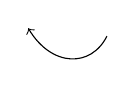
\begin{tikzpicture}[x=1cm,y=1cm]
\draw[->] (1,0)..controls(.8,-.4) and (.3,-.4)..(0,.1);
\end{tikzpicture}}
Pour ceci, nous allons définir un \uline{hom.\ en sens inverse}, et \uline{montrer que c'est un isomorphisme} (\unsure{cela en bonne dimension}!).

Or \deleted{\unsure{l'hom}}\inserted{donner} un \unsure{sens} inverse est équivalent à donner un accouplement
\margin{\textcircled{d}}
\[
\operatorname{pr}_1^*(F)\overset{\mathbb{L}}{\otimes}\operatorname{pr}_2^*\unsure{\underline{D}|D}_Y G_\bullet\overset{\mathbb{L}}{\otimes}\operatorname{pr}_2^*G\overset{\mathbb{L}}{\otimes}\operatorname{pr}_1^*\unsure{\underline{D}|D}_X(F_\bullet)\longrightarrow\deleted{\unsure{A}}K_Z^\bullet
\]
\margin{Plus explicite
\diagram{\begin{tikzcd}[ampersand replacement=\&,column sep=small]
\unsure{\mathbb{R}|\mathrm{R}}\mathcal{H}om^\bullet(\operatorname{pr}_1^*F,\operatorname{pr}_2^!G)\arrow[r]\&\unsure{\underline{D}|D}_Z\operatorname{pr}_1^*(F)\overset{\mathbb{L}}{\otimes}\operatorname{pr}_2^*(\unsure{\underline{D}|D}_Y G)\\
\unsure{\mathbb{R}|\mathrm{R}}\mathcal{H}om(\operatorname{pr}_1^*F,\operatorname{pr}_2^!G)\arrow[r]\&\unsure{\underline{D}|D}_Z\operatorname{pr}_2^*(G)\overset{\mathbb{L}}{\otimes}\operatorname{pr}_1^*(\unsure{\underline{D}|D}_X F)
\end{tikzcd}}
$\left.\vphantom{\begin{matrix}a\\b\end{matrix}}\right\}$ il faut accoupler les deuxièmes mb.\ \unsure{à valeurs} dans $K_Z^\bullet$.}
\margin{149}
